% -*- latex -*-
%%%%%%%%%%%%%%%%%%%%%%%%%%%%%%%%%%%%%%%%%%%%%%%%%%%%%%%%%%%%%%%%
%%%%%%%%%%%%%%%%%%%%%%%%%%%%%%%%%%%%%%%%%%%%%%%%%%%%%%%%%%%%%%%%
%%%%
%%%% This text file is part of the source of 
%%%% `Parallel Computing'
%%%% by Victor Eijkhout, copyright 2012-2021
%%%%
%%%% mpi_course.tex : master file for an MPI course
%%%%
%%%%%%%%%%%%%%%%%%%%%%%%%%%%%%%%%%%%%%%%%%%%%%%%%%%%%%%%%%%%%%%%
%%%%%%%%%%%%%%%%%%%%%%%%%%%%%%%%%%%%%%%%%%%%%%%%%%%%%%%%%%%%%%%%

\documentclass[11pt,headernav]{beamer}

\beamertemplatenavigationsymbolsempty
\usetheme{Madrid}%{Montpellier}
\usecolortheme{seahorse}
\setcounter{tocdepth}{1}

\setbeamertemplate{footline}{\hskip1em Eijkhout: MPI course\hfill
  \hbox to 0in {\hss 
\includegraphics[scale=.1]{tacclogonew}}%
  \hbox to 0in {\hss \arabic{page}\hskip 1in}}

\usepackage{multicol,multirow}
% custom arrays and tables
\usepackage{array} %,multirow,multicol}
\newcolumntype{R}{>{\hbox to 1.2em\bgroup\hss}{r}<{\egroup}}
\newcolumntype{T}{>{\hbox to 8em\bgroup}{c}<{\hss\egroup}}

\input commonmacs
\input slidemacs
\input coursemacs
\input listingmacs

\includecomment{full}
\excludecomment{condensed}
\excludecomment{online}

\specialcomment{tacc}{\stepcounter{tacc}\def\CommentCutFile{tacc\arabic{tacc}.cut}}{}
\newcounter{tacc}
%\excludecomment{tacc}
\excludecomment{xsede}

\includecomment{download}
\excludecomment{lab}

\includecomment{onesided}
\includecomment{advanced}
\includecomment{foundations}

\def\Location{}% redefine in the inex file
\def\courseyear{2021}
\def\Location{TACC APP institute MPI training \courseyear}
\def\Location{TACC/XSEDE MPI training \courseyear}
\def\Location{PEARC2020\\
  \url{http://tinyurl.com/tacc-pearc-2020}\\
  \texttt{\char126 train00/mpithree\_course\_2020.tgz}
}
\def\Location{ISS 2021}
\def\TitleExtra{}

%%%%
%%%% exercise stuff
%%%%
\usepackage{tocbasic}
\DeclareNewTOC[%
  type=programming,
  name=programming,
  listname={List of Exercises},
  ]{lox}

%%%%
%%%% save slides for separate MPI-3 lecture
%%%%
\newcounter{mpithree}
\specialcomment{mpithree}{
  \stepcounter{mpithree}
  \def\CommentCutFile{mpithree\arabic{mpithree}.cut}
  }{}
\excludecomment{mpitwo}

%%%%%%%%%%%%%%%%
%%%%%%%%%%%%%%%% Document
%%%%%%%%%%%%%%%%

\begin{document}
\parskip=10pt plus 5pt minus 3pt

\title{Advanced MPI and MPI-3}
\author{Victor Eijkhout {\tt eijkhout@tacc.utexas.edu}}
\date{\Location}

\begin{frame}
  \titlepage
\end{frame}

\begin{xsede}
  \input xsede-conduct
\end{xsede}

\begin{download}
  \begin{frame}[containsverbatim]{Materials}
    Textbook and lecture slides:\\
    \url{https://tinyurl.com/vle335course}
    
    Source repository containing exercises: \\
    \url{https://bitbucket.org/VictorEijkhout/parallel-programming-public/}
  \end{frame}
\end{download}

\begin{lab}
  \begin{frame}[containsverbatim]{Materials and labs}
    Textbook and lecture slides: \url{https://tinyurl.com/vle335course}

    Labs:
    \begin{itemize}
    \item Login
\begin{verbatim}
  ssh you@frontera.tacc.utexas.edu
\end{verbatim}

\item Get exercise material:\\
\begin{verbatim}
  tar fxz ~train00/mpithree_course_2021.tgz
\end{verbatim}

\item Pick your favorite language:\\
\begin{verbatim}
  cd mpithree_course/exercises-mpi-c
\end{verbatim}
  or \n{f08} or \n{p}
\item Get a compute node:
\begin{verbatim}
  idev -t 3:0:0
\end{verbatim}

\item Can you make an exercise?\\
\begin{verbatim}
  make hello && ibrun hello
\end{verbatim}

    \end{itemize}
  \end{frame}
\end{lab}

\begin{frame}{Justification}
  Version 3 of the MPI standard has added a number
  of features, some geared purely towards functionality,
  others with an eye towards efficiency at exascale.
\end{frame}

\Level 0 {Fortran bindings}

\lstset{language=Fortran}
\begin{numberedframe}{Overview}
  The Fortran interface to MPI had some defects.
  With Fortran2008 these have been largely repaired.
  \begin{itemize}
  \item The trailing error parameter is now optional;
  \item MPI data types are now actual \lstinline{Type} objects,
    rather than \lstinline{Integer}
  \item Strict type checking on arguments.
  \end{itemize}
\end{numberedframe}

\begin{numberedframe}{MPI headers}
\label{sl:mpi-header}
New module:
\begin{verbatim}
use mpi_f08   ! for Fortran2008
use mpi       ! for Fortran90
\end{verbatim}
True Fortran bindings as of the 2008 standard.
\begin{tacc}
Provided in Intel compiler version 18 or newer. Not in gcc7.
\end{tacc}
\end{numberedframe}

\begin{numberedframe}{Optional error parameter}
\lstset{language=Fortran}
\begin{lstlisting}
call MPI_Init()     ! F08 style
call MPI_Init(ierr) ! F90 style
! your code
call MPI_Finalize()     ! F08 style
call MPI_Finalize(ierr) ! F90 style
\end{lstlisting}
\end{numberedframe}

\begin{numberedframe}{Communicators}
\begin{lstlisting}
!! Fortran 2008 interface
use mpi_f08
Type(MPI_Comm) :: comm = MPI_COMM_WORLD
\end{lstlisting}
\begin{lstlisting}
!! Fortran legacy interface
#include <mpif.h>
! or: use mpi
Integer :: comm = MPI_COMM_WORLD
\end{lstlisting}
\end{numberedframe}

\begin{numberedframe}{Requests}
  Requests are also derived types\\
  note that \n{...NULL} entities are now objects, not integers

  \fverbatimsnippet{waitany0f}

  (Q for the alert student: do you see anything halfway
  remarkable about that index?)
\end{numberedframe}

\begin{numberedframe}{More}
\begin{lstlisting}
Type(MPI_Datatype) :: newtype ! F2008
Integer            :: newtype ! F90
\end{lstlisting}

Also:
  \lstinline{MPI_Comm}, \lstinline{MPI_Datatype},
  \lstinline{MPI_Errhandler}, \lstinline{MPI_Group},
  \lstinline{MPI_Info}, \lstinline{MPI_File}, \lstinline{MPI_Op},
  \lstinline{MPI_Request}, \lstinline{MPI_Status}, \lstinline{MPI_Win}
\end{numberedframe}

\begin{numberedframe}{Type checking}
  Type checking catches potential problems:
  \fverbatimsnippet{ftypecheck}
\begin{verbatim}
typecheck.F90(20): error #6285: 
  There is no matching specific subroutine
  for this generic subroutine call.   [MPI_SEND]
  call MPI_Send(source,n,MPI_INTEGER,1,0,MPI_COMM_WORLD)
-------^
\end{verbatim}
Unfortunately it doesn't say \emph{which} parameter is the offending one.
\end{numberedframe}

\lstset{language=C}

\Level 0 {Big data sends}
\input Bigdata-slides

\Level 0 {Atomic operations}
\input Atomic-slides
%\input{sl:fetchop}
 
\Level 0 {Non-blocking collectives}
\input Highercollective-slides

\Level 0 {Shared memory}
\input Sharedmemory-slides

\Level 0 {Process topologies}
\input Graph-slides

\Level 0 {Intercommunicator recap}
\begin{frame}{Inter-communicators}
\label{sl:comm-inter}
  \begin{itemize}
  \item Communicators so far are of \indextermsubh{intra}{communicator} type.
  \item Bridge between two communicators: \indextermsubh{inter}{communicator}.
  \item Example: communicator with newly spawned processes
  \end{itemize}
\end{frame}

\begin{frame}{In a picture}
\label{sl:intercomm-picture}
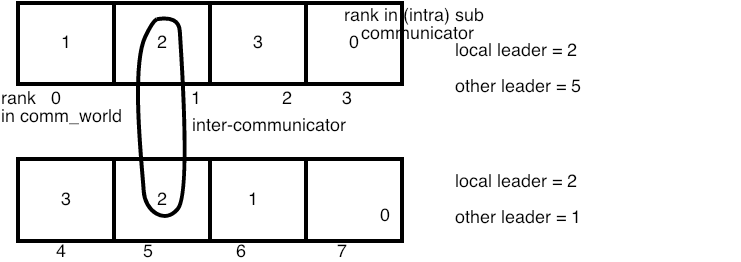
\includegraphics[scale=.4]{intercomm}

Illustration of ranks in an inter-communicator setup
\tiny\cverbatimsnippet{intercommcreate}
\end{frame}

\begin{frame}{Concepts}
\label{sl:intercomm-concepts}
\begin{itemize}
\item Two local communicators
\item The `peer' communicator that contains them
\item Leaders in each of them
\item An inter-communicator over the leaders.
\end{itemize}
\end{frame}

\begin{numberedframe}{Routines}
  \label{sl:intercomm-routines}
  \begin{itemize}
  \item
    \indexmpishow{MPI_Intercomm_create}: create
  \item \indexmpishow{MPI_Comm_get_parent}: the other leader (see process management)
  \item \indexmpishow{MPI_Comm_remote_size}, \indexmpishow{MPI_Comm_remote_group}:
    query the other communicator
  \item \indexmpishow{MPI_Comm_test_inter}: is this an inter or intra?
  \end{itemize}
\end{numberedframe}


\Level 0 {Process management}
\input Spawn-slides

\coursepart{Supplemental material}

\begin{comment}
  \begin{numberedframe}{Protocol}
    \label{sl:rendezvous}
    Communication is a `rendez-vous' or `hand-shake' protocol:
    \begin{itemize}
    \item Sender: `I have data for you'
    \item Receiver: `I have a buffer ready, send it over'
    \item Sender: `Ok, here it comes'
    \item Receiver: `Got it.'
    \end{itemize}
    Small messages bypass this: `eager' send.\\
    Definition of `small message' controlled by environment variables.
  \end{numberedframe}
\end{comment}

\begin{exerciseframe}[serialsend]
  \label{exserialsend}
  \input{ex:serialsend}
\end{exerciseframe}

\begin{exerciseframe}[procgrid]
  \label{ex:rowcolcomm}
  \input{ex:rowcolcomm}
\end{exerciseframe}

\end{document}

